\section{Burndown Chart}\label{sec:burndown}
The burndown chart seen below shows the current status of project after four sprints have been completed. It also shows the estimated progress of the project in its entirety. The blue line represents the actual progress and the red line the estimated progress.

\begin{figure}[H]
	\centering
	\graphicspath{ {./graphics/} }
    \centerline{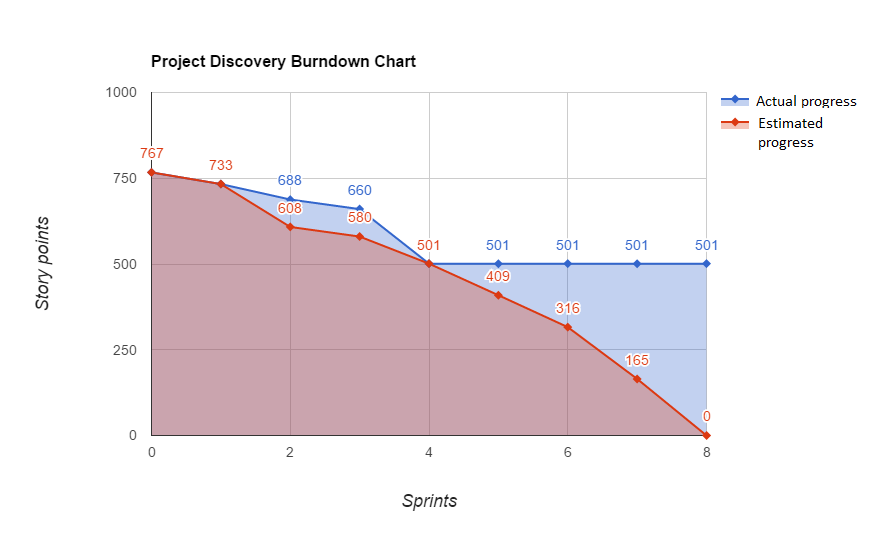
\includegraphics[scale=0.55]{bdc.png}}
    \caption{\label{fig:bdchart}The burndown chart after 4 sprints}
\end{figure}

The total story points for the project are now at 767 points. When we last handed in a progress report we had a total of 653 story points. Since then we have added some stories due to feedback from the preliminary user test. A total of 501 story points remain, of those story points, 298 belong to A stories. A typical base story would be "As a player, I can see my accuracy rating" which is a 13 point story which should take around 11 hours to complete. That story included tasks like implementing a fill for the accuracy meter, making the fill relate to a player's accuracy, and adding animations for the meter.

We estimated our velocity to be quite low for the first sprint since we figured it would take time to get acquainted with the project, the work environment and the tools we would need to work with. After that we estimated that our velocity would increase and average out to about 70 story points per sprint during the 12 week semester. After that our capacity will much higher since we can focus solely on the project so we estimated our velocity for the last two sprints to be 158 story points per sprint. 

So far our average velocity has been 66.5 story points per sprint and that includes a low velocity first sprint. If we keep up the same average velocity for the rest of the project that would result in 532 finished story points, which falls 32 story points shy of finishing all A stories. We are not worried about that however because of the greatly increased capacity we will have for the last two sprints which should bring our average up by a great amount. With that increased capacity we should be able to finish all A stories and hopefully most of the B and C stories.

